\documentclass[10pt,a4paper]{amsart}

\usepackage{amsmath}
\usepackage{physics}
\usepackage{listings}
\usepackage{graphicx}
\usepackage[]{hyperref}
\usepackage{float}

\lstset{
	frame = single,
	language = Python,
	showstringspaces = false,
	tabsize = 2,
	otherkeywords = {self},
	keywordstyle = \color{blue},
	identifierstyle=\color{deepgreen},
 	stringstyle=\color{orange},
 	backgroundcolor=\color{mygray}
}

\title[Rotation of Diatomic Molecules]{Rotation of Diatomic Molecules \\
	\hrulefill\fbox{FYS2160}\hrulefill}
	
\author[Winther-Larsen]{Sebastian G. Winther-Larsen\\
\href{https://github.com/gregwinther/FYS2160/}{\texttt{github.com/gregwinther}}}

\date{\today}

\begin{document}

\maketitle

\section{Introduction}
This study shows how to connect a microscopic and macroscopic representation of a canonical system, as system with given $N$, $V$ and $T$ (number of particles/molecules, volume of the system and temperature respectively). A general method can be applied to all canonical systems. First, finding the partition function. Second, one derives a function for Hermholtz free energy. Lastly, the remaining interesting aspects of the system can be found, like the entropy and heat capacity. All program code for this project can be found at the github address stated above.

\section{A simplified model system}
In this simple system we look at a diatomic molecule, which at low temperatures can be in four different states, $i=1,2,3,4$, with energies $\varepsilon_i=\varepsilon$, $\varepsilon_2=\varepsilon_3=\varepsilon_4=2\varepsilon$. In other words, this system has two possible energies, $\varepsilon$ and $2\varepsilon$. The highest energy has a degeneracy of $3$.

The partition function is found by the following formula
\begin{equation}
Z = \sum_ie^{-\beta E_i},\quad \beta=\frac{1}{kT},
\end{equation}
colloquially, the sum of a special transform called the Boltzmann factor of every state. For this system the partition function is
\begin{equation}
Z = e^{-\beta\varepsilon}+3e^{-2\beta\varepsilon}
\end{equation}
One could employ Hermholtz' free energy
\begin{equation}
F = E - TS= -kT\ln Z.
\end{equation}
First, computing
\begin{align*}
\ln Z &= \ln (e^{-\beta\varepsilon}+3e^{-2\beta\varepsilon} ) = \ln( e^{-\beta\varepsilon}) + \ln(1+3e^{-\beta\varepsilon} ) \\
&\approx ln( e^{-\beta\varepsilon}) + \ln(3e^{-\beta\varepsilon} )  = -\beta\varepsilon + \ln(3) -\beta\varepsilon  = -2\beta\varepsilon + \ln(3).
\end{align*}
The approximation on the second line might not strictily speaking be necessary because the expression for the partition function is simple enough as it is. Instead of going this way I will compute the average energy instead.

The average energy of this system can be found by differentiating $Z$ with respect to $\beta$, and multiplying by $-1/Z$.
\begin{equation}
\bar{E} = -\frac{1}{Z}\frac{\partial Z}{\partial \beta}=
\frac{\varepsilon e^{-\varepsilon\beta}+6\varepsilon e^{-2\varepsilon\beta} }{e^{-\varepsilon\beta} + 3e^{-\varepsilon\beta}} = \frac{\varepsilon(e^{exp(\varepsilon\beta}+6)}{e^{\varepsilon\beta}+3}.
\end{equation}
Because $\beta = 1/kT$ we have the energy as a function of temperature.

The heat capaciy, when no work is done on the system and volume is constant, is given by
\begin{equation}
C_V = \left(\frac{\partial E}{\partial T} \right)_V
\end{equation}
In this case, the heat capacity is 
\begin{equation*}
C_V =\left(\frac{\partial E}{\partial T} \right)_V =
\frac{3\varepsilon e^{\varepsilon/Tk}}{T^2k(e^{\varepsilon/Tk}+3)^2}
\end{equation*}

A plot of the heat capacity can be found in figure \ref{fig:heatcap1}. We see that the heat capacity quickly approaches zero for larger temperatures. This result is further underlined by the results shown in table \ref{tab:heatcap1}.

\begin{table}
	\caption{Heat capacity for the simple diatomic molecule system.}
	\begin{tabular}{rr} \hline
	T[K]  & C[J/K] \\ \hline 
	$  1$ & $8.8114\times10^5$ \\
	$ 25$ & $2.1152\times10^7$ \\
	$ 50$ & $5.1519\times10^8$ \\
	$100$ & $1.2707\times10^8$ \\
	$273$ & $1.6902\times10^9$ \\ \hline
	\end{tabular}
	\label{tab:heatcap1}
\end{table}

This system is not a very realistic system. There are very few moleucules involved, and the volume of the sytem is assumed to be unchanged as the temperature rises. One would assume that a system of gasseous nature would expand as the temperature increases. Furthermore, the temperature domain of the system is just arounda few degrees Kelvin at which most, if not all, substances are liquid. There are very few systems able to sustain temperatures this low\footnote{One example may be liquid helimum, which has a temperature of around 4 Kelvin}.

\begin{figure}
	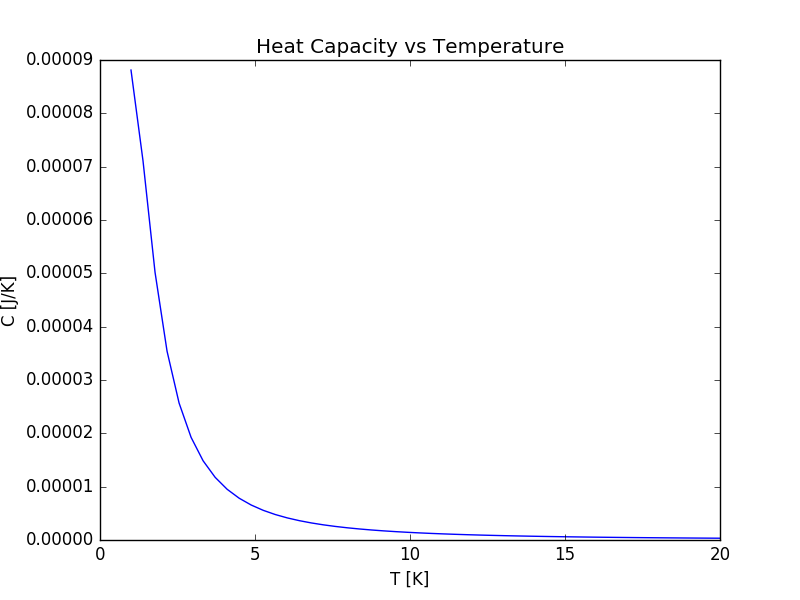
\includegraphics[width=0.9\textwidth]{figures/heatcapsimple.png}
	\caption{Plot of heat capacity vs temperature for the simple 			diatomic molecule system.}
	\label{fig:heatcap1}
\end{figure}

\section{Full model system of a rotating dimolecule}

For a diatomic molecule, the rotational energies are quantized inte energy levels described by $j$
\begin{equation}
\varepsilon_j=j(j+1)\theta_r k, \quad j=0,1,2,\dots
\end{equation}
where
\begin{equation}
\theta_r k= \frac{\hbar^2}{2I}
\end{equation}
where $I$ is the moment of intertia for the molecule. The values of $\theta_r$ for some molecules are listed in table \ref{tab:thetar}. The energy states are degenerate, and the degeneration of each energy given by $j$ is $d(j)=2j+1$.

\begin{table}
	\centering
	\caption{$\theta_r$ for different molecules}
	\begin{tabular}{ccccccc} \hline
 	 & $H_2$ & $HCl$ & $HI$ & $N_2$ & $Cl_2$ & $I_2$ \\ \hline
	$\theta_r(K)$ & 85.4 & 15.2 & 9.0 & 2.86 & 0.346 & 0.054 \\ \hline
	\end{tabular}
	\label{tab:thetar}
\end{table} 

The partition function for this system is
\begin{equation}
\label{eq:partition}
Z_{rot} = \sum_j (2j + 1)e^{-\beta\varepsilon_j} 
        = \sum_j (2j + 1)e^{-\beta j(j+1)\theta_r k}
        = \sum_j (2j + 1)e^{-j(j+1)\theta_r/T}
\end{equation}
Figure \ref{fig:partitionterms} shows the terms in the sum of this function for various values of $T/\theta_r$. The tendency ic clear: as the temperature $T$ gets higher relative to $theta_r$, the term $z(j)$ is more significant, especially as $j$ increases as well. If $T$ is small, relative to $\theta_r$, $z(t)$ quickly drops to zero for higher states $j$. 

\begin{figure}
	\centering
	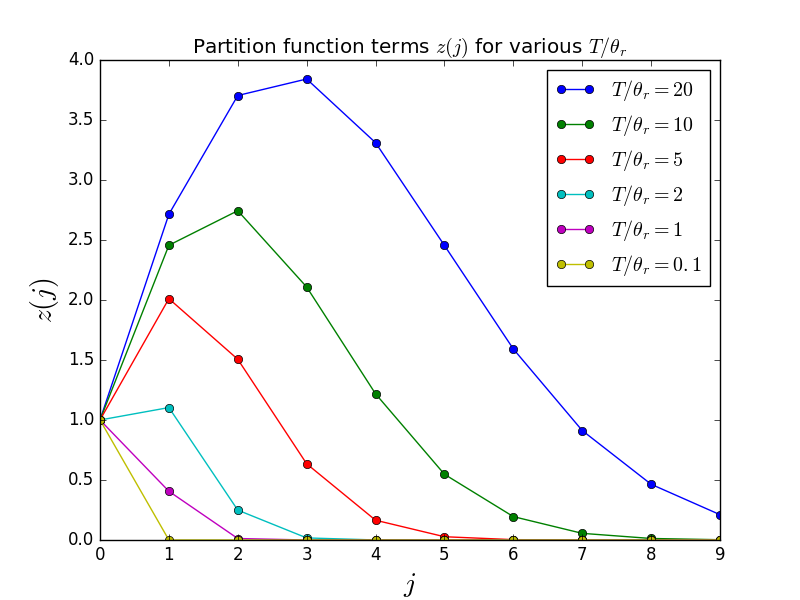
\includegraphics[width=0.9\textwidth]{figures/partitionterms.png}
	\caption{The terms in the partition function in equation \ref{eq:partition} for various values of $\frac{T}{\theta_r}$}
	\label{fig:partitionterms}
\end{figure}

The problem with the partition function in equation \ref{eq:partition} is that it difficult to evaluate a sum like this in closed form exactly. But for a sufficiently large $T/\theta_r$ one can approximate the sum with an integral.
\begin{equation}
Z_{rot} \approx \int_0^{\infty} (2j+1)e^{-j(j+1)\theta_r/T}dj
\end{equation}
This integral is realtively easy to solve by the substitution $x=j(j+1)\theta_r/T$ and $dx = (2j+1)\theta_r dj/T$ which gives
\begin{equation}
\frac{T}{\theta_r}\int_0^{\infty}e^{-x}dx=\frac{T}{\theta_r}
\end{equation}
Well, what do you know? A (perhaps not so) suprisingly simple and nice expression fell out.

On the other hand, we have the opposite situation where $T << \theta_r$. It is sufficient to only look at the first few terms within the sum of the partition function (equation \ref{eq:partition}) in this case (e.g. $j=0,1,2,3$)
\begin{equation}
Z_{rot} \approx 1+e^{-\theta_r/T}+3e^{-2\theta_r/T}+5e^{-6\theta_r/T}+7e^{-12\theta_r/T}
\end{equation}
which for the borderline case $T=\theta_r$ will form a convergent series\footnote{This is easy to check with the ratio test, where one would formulate the test limit $L=\lim_{n\to\infty}\abs{a_{n+1}/a_n}$. If $L<1$ the series converges absolutely.}
\begin{equation*}
Z_{rot} \approx 1 + \frac{3}{e^2}+\frac{5}{e^6}+\frac{7}{e^{12}} + \dots \approx 1 + 0.406006 + 0.012394 + 0.0000430 + \dots \approx 1.41844
\end{equation*}
while for the case $T >> \theta_r$, all terms except the first one will disappear and we get
\begin{equation*}
Z_{rot} = 1
\end{equation*}


\end{document}